\documentclass{standalone}
\usepackage{tikz}
\usetikzlibrary{patterns, positioning}

\begin{document}
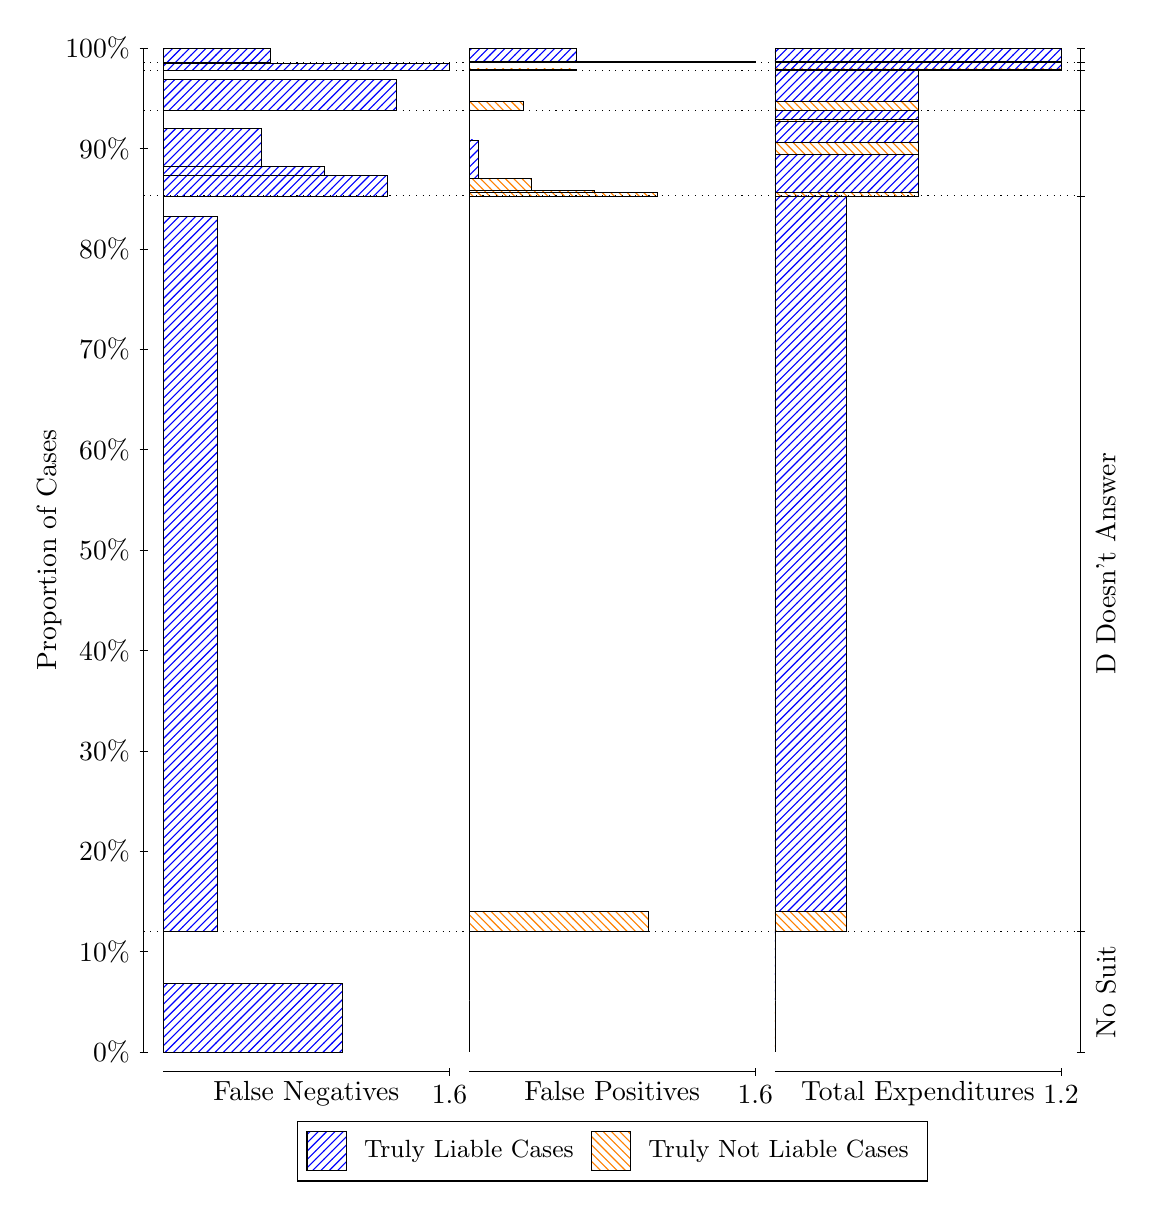
\begin{tikzpicture}
\draw[black, very thin] (1.5,1.75) -- (1.5,14.5);
\node[rotate=90, anchor=center] at (0.3, 8.125) {Proportion of Cases};
\draw[black, very thin] (1.45,1.75) -- (1.55,1.75);
\node[anchor=east] at (1.45, 1.75) {0\%};
\draw[black, very thin] (1.45,3.025) -- (1.55,3.025);
\node[anchor=east] at (1.45, 3.025) {10\%};
\draw[black, very thin] (1.45,4.3) -- (1.55,4.3);
\node[anchor=east] at (1.45, 4.3) {20\%};
\draw[black, very thin] (1.45,5.575) -- (1.55,5.575);
\node[anchor=east] at (1.45, 5.575) {30\%};
\draw[black, very thin] (1.45,6.85) -- (1.55,6.85);
\node[anchor=east] at (1.45, 6.85) {40\%};
\draw[black, very thin] (1.45,8.125) -- (1.55,8.125);
\node[anchor=east] at (1.45, 8.125) {50\%};
\draw[black, very thin] (1.45,9.4) -- (1.55,9.4);
\node[anchor=east] at (1.45, 9.4) {60\%};
\draw[black, very thin] (1.45,10.675) -- (1.55,10.675);
\node[anchor=east] at (1.45, 10.675) {70\%};
\draw[black, very thin] (1.45,11.95) -- (1.55,11.95);
\node[anchor=east] at (1.45, 11.95) {80\%};
\draw[black, very thin] (1.45,13.225) -- (1.55,13.225);
\node[anchor=east] at (1.45, 13.225) {90\%};
\draw[black, very thin] (1.45,14.5) -- (1.55,14.5);
\node[anchor=east] at (1.45, 14.5) {100\%};

\draw[black, very thin] (13.4,1.75) -- (13.4,14.5);
\draw[black, very thin] (13.35,1.75) -- (13.45,1.75);
\node[anchor=west] at (13.35, 1.75) {};
\draw[black, very thin] (13.35,3.2774) -- (13.45,3.2774);
\node[anchor=west] at (13.35, 3.2774) {};
\draw[black, very thin] (13.35,12.622) -- (13.45,12.622);
\node[anchor=west] at (13.35, 12.622) {};
\draw[black, very thin] (13.35,13.706) -- (13.45,13.706);
\node[anchor=west] at (13.35, 13.706) {};
\draw[black, very thin] (13.35,14.219) -- (13.45,14.219);
\node[anchor=west] at (13.35, 14.219) {};
\draw[black, very thin] (13.35,14.32) -- (13.45,14.32);
\node[anchor=west] at (13.35, 14.32) {};
\draw[black, very thin] (13.35,14.5) -- (13.45,14.5);
\node[anchor=west] at (13.35, 14.5) {};

\draw[black, very thin, pattern color=blue, pattern=north east lines] (1.75,1.75) rectangle (4.0208,2.622);
\draw[black, very thin, pattern color=orange, pattern=north west lines] (1.75,2.622) rectangle (1.75,3.2774);
\draw[black, very thin, pattern color=blue, pattern=north east lines] (1.75,3.2774) rectangle (2.4312,12.364);
\draw[black, very thin, pattern color=orange, pattern=north west lines] (1.75,12.364) rectangle (1.75,12.622);
\draw[black, very thin, pattern color=blue, pattern=north east lines] (1.75,12.622) rectangle (4.5885,12.885);
\draw[black, very thin, pattern color=blue, pattern=north east lines] (1.75,12.885) rectangle (3.7937,12.997);
\draw[black, very thin, pattern color=blue, pattern=north east lines] (1.75,12.997) rectangle (2.999,13.484);
\draw[black, very thin, pattern color=orange, pattern=north west lines] (1.75,13.484) rectangle (1.75,13.706);
\draw[black, very thin, pattern color=blue, pattern=north east lines] (1.75,13.706) rectangle (4.7021,14.105);
\draw[black, very thin, pattern color=orange, pattern=north west lines] (1.75,14.105) rectangle (1.75,14.219);
\draw[black, very thin, pattern color=blue, pattern=north east lines] (1.75,14.219) rectangle (5.3833,14.304);
\draw[black, very thin, pattern color=orange, pattern=north west lines] (1.75,14.304) rectangle (1.75,14.32);
\draw[black, very thin, pattern color=blue, pattern=north east lines] (1.75,14.32) rectangle (3.1125,14.491);
\draw[black, very thin, pattern color=orange, pattern=north west lines] (1.75,14.491) rectangle (1.75,14.5);
\draw[black, very thin, pattern color=orange, pattern=north west lines] (5.6333,1.75) rectangle (5.6333,2.4054);
\draw[black, very thin, pattern color=blue, pattern=north east lines] (5.6333,2.4054) rectangle (5.6333,3.2774);
\draw[black, very thin, pattern color=orange, pattern=north west lines] (5.6333,3.2774) rectangle (7.9042,3.5349);
\draw[black, very thin, pattern color=blue, pattern=north east lines] (5.6333,3.5349) rectangle (5.6333,12.622);
\draw[black, very thin, pattern color=orange, pattern=north west lines] (5.6333,12.622) rectangle (8.0177,12.666);
\draw[black, very thin, pattern color=orange, pattern=north west lines] (5.6333,12.666) rectangle (7.2229,12.695);
\draw[black, very thin, pattern color=orange, pattern=north west lines] (5.6333,12.695) rectangle (6.4281,12.844);
\draw[black, very thin, pattern color=blue, pattern=north east lines] (5.6333,12.844) rectangle (5.7469,13.332);
\draw[black, very thin, pattern color=blue, pattern=north east lines] (5.6333,13.332) rectangle (5.6333,13.706);
\draw[black, very thin, pattern color=orange, pattern=north west lines] (5.6333,13.706) rectangle (6.3146,13.821);
\draw[black, very thin, pattern color=blue, pattern=north east lines] (5.6333,13.821) rectangle (5.6333,14.219);
\draw[black, very thin, pattern color=orange, pattern=north west lines] (5.6333,14.219) rectangle (6.9958,14.236);
\draw[black, very thin, pattern color=blue, pattern=north east lines] (5.6333,14.236) rectangle (5.6333,14.32);
\draw[black, very thin, pattern color=orange, pattern=north west lines] (5.6333,14.32) rectangle (9.2667,14.33);
\draw[black, very thin, pattern color=blue, pattern=north east lines] (5.6333,14.33) rectangle (6.9958,14.5);
\draw[black, very thin, pattern color=orange, pattern=north west lines] (9.5167,1.75) rectangle (9.5167,2.4054);
\draw[black, very thin, pattern color=blue, pattern=north east lines] (9.5167,2.4054) rectangle (9.5167,3.2774);
\draw[black, very thin, pattern color=orange, pattern=north west lines] (9.5167,3.2774) rectangle (10.425,3.5349);
\draw[black, very thin, pattern color=blue, pattern=north east lines] (9.5167,3.5349) rectangle (10.425,12.622);
\draw[black, very thin, pattern color=orange, pattern=north west lines] (9.5167,12.622) rectangle (11.333,12.666);
\draw[black, very thin, pattern color=blue, pattern=north east lines] (9.5167,12.666) rectangle (11.333,13.154);
\draw[black, very thin, pattern color=orange, pattern=north west lines] (9.5167,13.154) rectangle (11.333,13.303);
\draw[black, very thin, pattern color=blue, pattern=north east lines] (9.5167,13.303) rectangle (11.333,13.566);
\draw[black, very thin, pattern color=orange, pattern=north west lines] (9.5167,13.566) rectangle (11.333,13.595);
\draw[black, very thin, pattern color=blue, pattern=north east lines] (9.5167,13.595) rectangle (11.333,13.706);
\draw[black, very thin, pattern color=orange, pattern=north west lines] (9.5167,13.706) rectangle (11.333,13.821);
\draw[black, very thin, pattern color=blue, pattern=north east lines] (9.5167,13.821) rectangle (11.333,14.219);
\draw[black, very thin, pattern color=orange, pattern=north west lines] (9.5167,14.219) rectangle (13.15,14.236);
\draw[black, very thin, pattern color=blue, pattern=north east lines] (9.5167,14.236) rectangle (13.15,14.32);
\draw[black, very thin, pattern color=orange, pattern=north west lines] (9.5167,14.32) rectangle (13.15,14.33);
\draw[black, very thin, pattern color=blue, pattern=north east lines] (9.5167,14.33) rectangle (13.15,14.5);
\draw[black, dotted] (1.5,3.2774) -- (13.4,3.2774);
\draw[black, dotted] (1.5,12.622) -- (13.4,12.622);
\draw[black, dotted] (1.5,13.706) -- (13.4,13.706);
\draw[black, dotted] (1.5,14.219) -- (13.4,14.219);
\draw[black, dotted] (1.5,14.32) -- (13.4,14.32);
\draw[black, very thin] (1.75,1.5) -- (5.3833,1.5);
\node[anchor=north] at (3.5667, 1.5) {False Negatives};
\draw[black, very thin] (5.3833,1.45) -- (5.3833,1.55);
\node[anchor=north] at (5.3833, 1.45) {1.6};

\draw[black, very thin] (5.6333,1.5) -- (9.2667,1.5);
\node[anchor=north] at (7.45, 1.5) {False Positives};
\draw[black, very thin] (9.2667,1.45) -- (9.2667,1.55);
\node[anchor=north] at (9.2667, 1.45) {1.6};

\draw[black, very thin] (9.5167,1.5) -- (13.15,1.5);
\node[anchor=north] at (11.333, 1.5) {Total Expenditures};
\draw[black, very thin] (13.15,1.45) -- (13.15,1.55);
\node[anchor=north] at (13.15, 1.45) {1.2};

\node[black, centered, rotate=90] at (13.72, 2.5137) {No Suit};
\node[black, centered, rotate=90] at (13.72, 7.9497) {D Doesn't Answer};





\draw (7.449999999999999,1.5) node[draw=none] (baseCoordinate) {};
\begin{scope}[align=center]
        \matrix[scale=0.5, draw=black, below=0.5cm of baseCoordinate, nodes={draw}, column sep=0.1cm]{
            \node[rectangle, draw, minimum width=0.5cm, minimum height=0.5cm, pattern=north east lines, pattern color=blue] {}; &
            \node[draw=none, font=\small] (B) {Truly Liable Cases}; &
            \node[rectangle, draw, minimum width=0.5cm, minimum height=0.5cm, pattern=north west lines, pattern color=orange] {}; &
            \node[draw=none, font=\small] (B) {Truly Not Liable Cases}; \\
            };
\end{scope}

\end{tikzpicture}
\end{document}